\chapter{Universal Module}\label{chap:universal_module}

\todo{Intro}

The universal RoFI module occupies two neighboring cubes of the grid as can be
seen in the figure \ref{fig:rofi_reference}. Please note that this drawing gives
a simplified model in which many technical details are omitted. There are four
parts from which the module is composed:
\begin{enumerate*}
    \item \emph{body A},
    \item \emph{body B},
    \item \emph{shoe A} and
    \item \emph{shoe B}.
\end{enumerate*}
See figure \ref{fig:rofi_body_parts}. Bodies are supposed to encapsulate
actuators, electronics and accumulators; shoes are meant to provide connection
to other modules and provide movement.

\begin{figure}
    \centering
    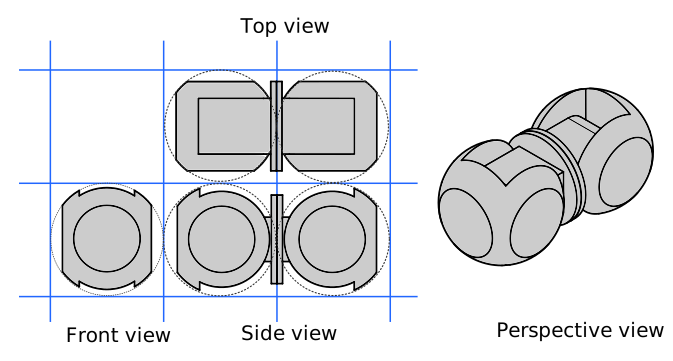
\includegraphics[width=\textwidth]{figures/rofi_reference.pdf}
    \caption{The universal RoFI module. Blue lines specify the grid, dotted
    lines marks spheres in which the module in inscribed. }
    \label{fig:rofi_reference}
\end{figure}

\begin{figure}
    \centering
    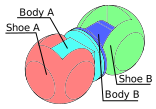
\includegraphics[width=0.7\textwidth]{figures/rofi_body_parts.pdf}
    \caption{Parts of the universal module.}
    \label{fig:rofi_body_parts}
\end{figure}

There are 3 degrees of freedom (figure \ref{fig:rofi_axis}):
\begin{enumerate*}
    \item shoe A can rotate against body A along the $\alpha$ axe in a range
    $\langle -90^\circ; +90^\circ\rangle$,
    \item shoe B can rorate against body B along the $\beta$ axe in a range
    $\langle -90^\circ; +90^\circ\rangle$ and
    \item body A can rotate against body B along the $\gamma$ axe in $\langle
    -180^\circ; +180^\circ\rangle$ with an overflow\footnote{First prototypes
    feature a limitation on a number of overflows in one direction the $\gamma$
    axe due to technical limitations. }.
\end{enumerate*}
The module should be able to provide at least 1.5 $\text{N}\cdot\text{m}$ of
torque for each axe.

\begin{figure}
    \centering
    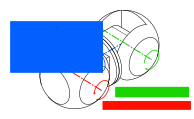
\includegraphics[width=0.7\textwidth]{figures/rofi_axis.pdf}
    \caption{Degrees of freedom of the universal module. The figure represents neutral position of each joint.}
    \label{fig:rofi_axis}
\end{figure}

The flat faces of shoes feature docking system for establishing mechanical
connection to other modules. There are 6 docks in total (figure
\ref{fig:rofi_locks}); 3 on each shoe. The docks are marked by the name of a
shoe and by one of following suffixes: $-1$, $0$, $1$. When facing the dock, its
index gives a factor by which we multiply degree of rotation to turn a shoe
around its axe in counter clockwise direction. Each dock is oriented. We denote
the orientation with an orientation vector. The vector starts in a middle of the
dock. The dock orientation is important for describing configurations of a
system (more detail on that can be found in section \ref{sec:configuration}).
Details about docking mechanism are given in section \ref{subsec:lock}.

\begin{figure}
    \centering
    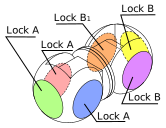
\includegraphics[width=0.7\textwidth]{figures/rofi_locks.pdf}
    \caption{Docks on the universal module. The arrow on each dock specifies its orientation.}
    \label{fig:rofi_locks}
\end{figure}

As it can be seen from the figures \ref{fig:rofi_reference} and
\ref{fig:rofi_body_parts}, the module does not occupy the whole space provided
by the grid. The module is (nearly) inscribed to two spheres (marked by a dotted
line in the figure \ref{fig:rofi_reference}). This allow the module to move its
shoe even if all neighbouring grid cells are occupied. We refer to this property
as \emph{grid-awareness}. This allows the module reconfigure more easily in
densely occupied grid -- see figure \ref{fig:grid_aware} for an example of such
a situation. Another perspective on grid-awareness of the universal module is
that no matter what position it is in, it never outreaches shape specified in
the figure \ref{fig:rofi_grid}.

\begin{figure}
    \centering
    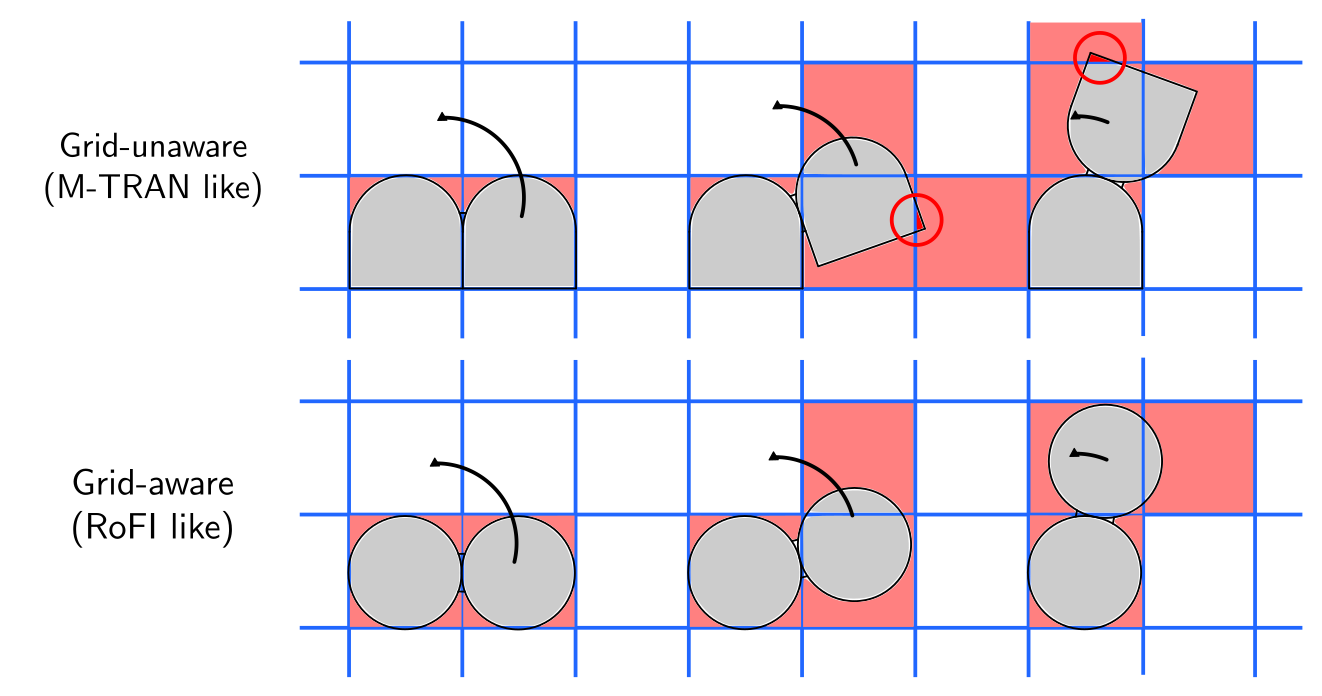
\includegraphics[width=\textwidth]{figures/grid_aware.pdf}
    \caption{Visualization of grid-awareness. Consider two module shapes -- M-TRAN\cite{haruhisa_kurokawa_m-tran_2003}
     like (int the top row) and RoFI like (in the bottom row). Given the task to
     move right body over the left one, M-TRAN like module occupies extra cells
     due to small parts of it body overlapping out of the gird. On the other
     hand, RoFI like module occupies the least cells required to make the
     movement.   }
    \label{fig:grid_aware}
\end{figure}

\begin{figure}
    \centering
    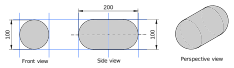
\includegraphics[width=\textwidth]{figures/rofi_grid.pdf}
    \caption{Reference shape for grid-awareness. If the module can be always inscribed in the shape, it is grid-aware.}
    \label{fig:rofi_grid}
\end{figure}

The grid-awareness prevents a face to face contact between two universal
modules. If the modules dock directly face to face, they would not fit in grid.
If the modules fully utilize the space allowed by the reference shape (figure
\ref{fig:rofi_grid}), they would feature only a point contact as two spheres
have only a single point touch. Therefore, there is a need for retractable
docking system. The docking system is specified in section \ref{subsec:lock}.
Here we only describe its relation to the grid.

If the module does not dock with another module, the dock is retracted in the
module shoe and therefore, the module does not outreach the reference shape.
When two modules dock to each other, the docks expand and connect to each other.
As the modules are now connected and no motion between them can be performed,
the enlarged footprint of module over the reference shape does not matter.
Illustration of the docking process can be found in the figure
\ref{fig:rofi_locking_example}.

\begin{figure}
    \centering
    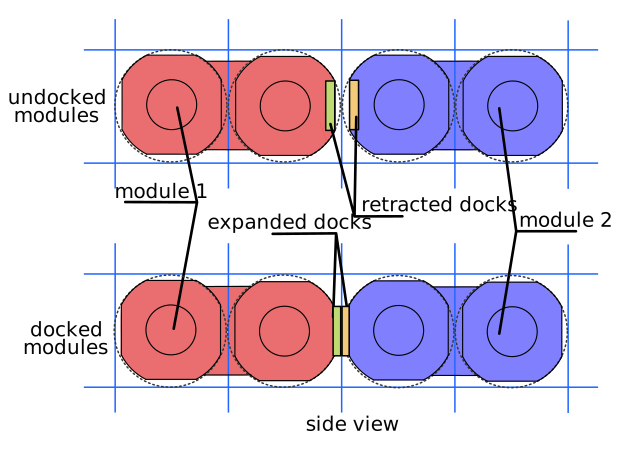
\includegraphics[width=\textwidth]{figures/rofi_locking_example.pdf}
    \caption{Docking procedure. There is a by-default retracted docking system
    in the module which expands when the docking should be performed.}
    \label{fig:rofi_locking_example}
\end{figure}

\subsection{Intramodule Architecture}

\subsection{The RoFI "BIOS" \todo{Proper naming}}

\subsection{RoFI lib}

\todo{Something here}